\documentclass[10pt]{report}
\usepackage{amsmath}
\usepackage{latexsym}
\usepackage{amsfonts}
\usepackage[normalem]{ulem}
\usepackage{soul}
\usepackage{array}
\usepackage{amssymb}
\usepackage{extarrows}
\usepackage{graphicx}
\usepackage[backend=biber,
style=numeric,
sorting=none,
isbn=false,
doi=false,
url=false,
]{biblatex}\addbibresource{bibliography-biblatex.bib}

\usepackage{subfig}
\usepackage{wrapfig}
\usepackage{txfonts}
\usepackage{wasysym}
\usepackage{enumitem}
\usepackage{adjustbox}
\usepackage{ragged2e}
\usepackage[svgnames,table]{xcolor}
\usepackage{tikz}
\usepackage{longtable}
\usepackage{changepage}
\usepackage{setspace}
\usepackage{hhline}
\usepackage{multicol}
\usepackage{tabto}
\usepackage{float}
\usepackage{multirow}
\usepackage{makecell}
\usepackage{fancyhdr}
\usepackage[toc,page]{appendix}
\usepackage[hidelinks]{hyperref}
\usetikzlibrary{shapes.symbols,shapes.geometric,shadows,arrows.meta}
\tikzset{>={Latex[width=1.5mm,length=2mm]}}
\usepackage{flowchart}\usepackage[paperheight=11.0in,paperwidth=8.5in,left=1.0in,right=1.0in,top=1.5in,bottom=1.5in,headheight=1in]{geometry}
\usepackage[utf8]{inputenc}
\usepackage[T1]{fontenc}
\TabPositions{0.5in,1.0in,1.5in,2.0in,2.5in,3.0in,3.5in,4.0in,4.5in,5.0in,5.5in,6.0in,}

\urlstyle{same}


 %%%%%%%%%%%%  Set Depths for Sections  %%%%%%%%%%%%%%

% 1) Section
% 1.1) SubSection
% 1.1.1) SubSubSection
% 1.1.1.1) Paragraph
% 1.1.1.1.1) Subparagraph


\setcounter{tocdepth}{5}
\setcounter{secnumdepth}{5}


 %%%%%%%%%%%%  Set Depths for Nested Lists created by \begin{enumerate}  %%%%%%%%%%%%%%


\setlistdepth{9}
\renewlist{enumerate}{enumerate}{9}
		\setlist[enumerate,1]{label=\arabic*)}
		\setlist[enumerate,2]{label=\alph*)}
		\setlist[enumerate,3]{label=(\roman*)}
		\setlist[enumerate,4]{label=(\arabic*)}
		\setlist[enumerate,5]{label=(\Alph*)}
		\setlist[enumerate,6]{label=(\Roman*)}
		\setlist[enumerate,7]{label=\arabic*}
		\setlist[enumerate,8]{label=\alph*}
		\setlist[enumerate,9]{label=\roman*}

\renewlist{itemize}{itemize}{9}
		\setlist[itemize]{label=$\cdot$}
		\setlist[itemize,1]{label=\textbullet}
		\setlist[itemize,2]{label=$\circ$}
		\setlist[itemize,3]{label=$\ast$}
		\setlist[itemize,4]{label=$\dagger$}
		\setlist[itemize,5]{label=$\triangleright$}
		\setlist[itemize,6]{label=$\bigstar$}
		\setlist[itemize,7]{label=$\blacklozenge$}
		\setlist[itemize,8]{label=$\prime$}

\setlength{\topsep}{0pt}\setlength{\parindent}{0pt}

 %%%%%%%%%%%%  This sets linespacing (verticle gap between Lines) Default=1 %%%%%%%%%%%%%%


\renewcommand{\arraystretch}{1.3}

\title{\ \ \ \  Design and Analysis of Algorithms}
\date{}


%%%%%%%%%%%%%%%%%%%% Document code starts here %%%%%%%%%%%%%%%%%%%%



\begin{document}

\maketitle

{\fontsize{15pt}{18.0pt}\selectfont \textbf{C2 Assignment-3},\textbf{Group-3}}

\vspace{\baselineskip}
\ \ \ \ \ \  \tab  Rahul Roy\ \ \ \ \ \ \ \ \ \ \ \ \ \ \ \ \ \ \  \tab \ \ \ \ \ \ \ \ \  \tab \ \ \ \ \  Chetan Patidar\ \ \ \ \ \ \ \ \ \ \  \tab \ \ \ \ \  Pritik Shrivastava 
\ \ \ \ \ \ \ \ \ \ \ \ \  IIT2019194\ \ \ \ \ \ \ \ \ \ \ \ \ \ \ \ \ \ \ \ \ \ \ \ \ \ \ \ \ \ \ \ \ \ \ \ \ \ \ \ \ IIT2019191\ \ \ \ \ \ \ \ \ \ \ \ \ \ \ \ \ \ \ \ \ \ \ \ \ \ \ \ \ \ \   IIT2019192

\vspace{\baselineskip}
\begin{multicols}{2}

\vspace{\baselineskip}
\setlength{\parskip}{5.0pt}
{\fontsize{9pt}{10.8pt}\selectfont \textbf{Abstract-}}\textcolor[HTML]{40424E}{Given n number of sorted files, the task is to find the minimum computations done to reach Optimal Merge Pattern. When two or more sorted files are to be merged all together to form a single file, the minimum computations done to reach this file are known as Optimal Merge Pattern.}
{\fontsize{9pt}{10.8pt}\selectfont \textbf{. }}

\vspace{\baselineskip}
{\fontsize{9pt}{10.8pt}\selectfont \textbf{\ \ \ \ \ \ \ \ \ \ \ \  }}\textbf{ \  I. INTRODUCTION}

\vspace{\baselineskip}
In simple words, the problem can be explained as follows:
We are given n sorted files and we need to find the total number of minimum computations required to reach Optimal Merge Pattern.\textcolor[HTML]{40424E}{ If more than 2 files need to be merged then it can be done in pairs. For example, if need to merge 4 files A, B, C, D. First Merge A with B to get X1, merge X1 with C to get X2, merge X2 with D to get X3 as the output file.}
\setlength{\parskip}{0.0pt}
If we have two files of sizes m and n, the total computation time will be m+n. Here, we use \href{https://www.geeksforgeeks.org/greedy-algorithms/}{greedy} strategy by merging two smallest size files among all the files present.

\vspace{\baselineskip}
We will solve the given problem using greedy approach
This report further contains -

\vspace{\baselineskip}
II. Algorithm Design
III. Algorithm Analysis
IV. Experimental Study
V. Conclusion

\vspace{\baselineskip}

\vspace{\baselineskip}
\ \ \ \ \  \textbf{\ \ \ \ \ \ \  II.A}{\fontsize{9pt}{10.8pt}\selectfont \textbf{LGORITHM DESIGN}}

\vspace{\baselineskip}
\textcolor[HTML]{40424E}{Firstly we add all the nodes in a priority queue (Min Heap) where node.weight = file size and given nodes are greater than 2}
\textcolor[HTML]{40424E}{Then we initiate the process by initializing count = 0 which is the variable to store file computations.}

\vspace{\baselineskip}
\textbf{1.}An array of files is created storing the size of each file in a sorted manner.

\vspace{\baselineskip}
\textbf{2. }The priority queue is created to handle each iteration over each file.

\vspace{\baselineskip}
\textbf{3. }In each iteration we find the two files with minimum sizes and merge them into one and store it.

\vspace{\baselineskip}
\textbf{4}. Then in every next iteration we merge the current file into the previous merged file

\vspace{\baselineskip}
\textbf{5.} In this way we compute the total number of iterations required to reach optimal merge pattern.

\vspace{\baselineskip}

\vspace{\baselineskip}
\textbf{For example-}

\vspace{\baselineskip}
\textbf{Consider input array as follows:-}
\textbf{\textcolor[HTML]{40424E}{Input:}}\textcolor[HTML]{40424E}{ n = 3, size = $ \{ $ 2, 3, 4$ \} $ }
Firstly we merge 2 and 3 into one file of size 5. Then the next is 4. So we merge file with size 4 with the previously merged file of size 5 to get 4+5=9.
Hence total cost = 14

\vspace{\baselineskip}

\vspace{\baselineskip}

\vspace{\baselineskip}

\vspace{\baselineskip}

\vspace{\baselineskip}

\vspace{\baselineskip}

\vspace{\baselineskip}

\vspace{\baselineskip}

\vspace{\baselineskip}

\vspace{\baselineskip}

\vspace{\baselineskip}

\vspace{\baselineskip}

\vspace{\baselineskip}

\vspace{\baselineskip}

\vspace{\baselineskip}
\ \  
\textcolor[HTML]{40424E}{Repeat while the size of priority Queue is greater than 1. Now we create a new node such that :}
\textcolor[HTML]{40424E}{new node = pq.poll().weight+pq.poll().weight;}
\textcolor[HTML]{40424E}{where pq denotes priority queue, remove 1st smallest and 2nd smallest element and add their weights to get a new node}
\begin{enumerate}
	\item \textcolor[HTML]{40424E}{count = count + node.weight}
	\item \textcolor[HTML]{40424E}{add this new node to priority queue;}
\end{enumerate}
\textcolor[HTML]{40424E}{Hence we get count as the final answer}
\textcolor[HTML]{40424E}{For example lets say we have  n = 6 }
\textcolor[HTML]{40424E}{size = $ \{ $ 2, 3, 4, 5, 6, 7$ \} $ , then by use of the above discussed algorithm we have final count = 68.}

\vspace{\baselineskip}


%%%%%%%%%%%%%%%%%%%% Figure/Image No: 1 starts here %%%%%%%%%%%%%%%%%%%%

\begin{figure}[H]
	\begin{Center}
		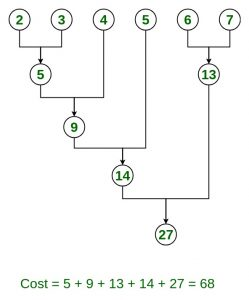
\includegraphics[width=2.59in,height=3.12in]{./media/image1.jpeg}
	\end{Center}
\end{figure}


%%%%%%%%%%%%%%%%%%%% Figure/Image No: 1 Ends here %%%%%%%%%%%%%%%%%%%%


\vspace{\baselineskip}
\vspace{\baselineskip}
\textbf{\ \ \ \ \ \ \ \ \  }

\vspace{\baselineskip}
\textbf{\ \ \ \ \ \ \ \ \ \ \ \ \  \  \  PSEUDO CODE}

\vspace{\baselineskip}

\vspace{\baselineskip}
{\fontsize{12pt}{14.4pt}\selectfont \textbf{ A}lgorithm}{\fontsize{12pt}{14.4pt}\selectfont  minimumComputation}
{\fontsize{12pt}{14.4pt}\selectfont  \textbf{P}assed}{\fontsize{12pt}{14.4pt}\selectfont  vector<int> files}

\vspace{\baselineskip}

\vspace{\baselineskip}

\vspace{\baselineskip}
while(!q.empty())
\ \ \ \ $ \{ $ \   
\ \ \ \ \ \ \  ll x=-1$\ast$ q.top();
\ \ \ \ \ \ \  q.pop();
\ \ \ \ \ \ \  if(q.empty())
\ \ \ \ \ \ \ \ \ \ \  break;
\ \ \ \ \ \ \  ll y=-1$\ast$ q.top();
\ \ \ \ \ \ \  q.pop();
 
\ \ \ \ \ \ \  ans+=x+y;
\ \ \ \ \ \ \ \ q.push(  -1$\ast$ (x+y) );

\vspace{\baselineskip}
\ \ \  $ \} $ 

\vspace{\baselineskip}

\vspace{\baselineskip}

\vspace{\baselineskip}

\vspace{\baselineskip}

\vspace{\baselineskip}

\vspace{\baselineskip}

\vspace{\baselineskip}

\vspace{\baselineskip}

\vspace{\baselineskip}

\vspace{\baselineskip}

\vspace{\baselineskip}

\vspace{\baselineskip}
\textbf{\ \ \ \ \ \ \ \ \ \   III.ALGORITHM ANALYSIS}

\vspace{\baselineskip}
\textbf{A. Time complexity}

\vspace{\baselineskip}
The\textbf{ A}lgorithm uses minheap to provide a greedy solution. 
The algorithm takes into account the two minimum elements or file sizes present in the array or vector in O(logn) and then iterates for n-1 elements to find this which takes O(n).
So overall time complexity of the algorithm becomes O(nlogn).

\vspace{\baselineskip}
\textbf{B.\ Space\ complexity\    \ \ \ \ \  }

\vspace{\baselineskip}
The space complexity of the program is \textbf{O(n)} as we store the size of n files.

\vspace{\baselineskip}

\vspace{\baselineskip}

\vspace{\baselineskip}

\vspace{\baselineskip}

\vspace{\baselineskip}

\vspace{\baselineskip}

\vspace{\baselineskip}

\vspace{\baselineskip}

\vspace{\baselineskip}

\vspace{\baselineskip}

\vspace{\baselineskip}
\textbf{\ \ \ \ \ \ \ \  \  IV. EXPERIMENTAL STUDY\  }

\vspace{\baselineskip}
\textbf{Graph(Fig .1) }From the graph plotted between the n(no. of rows :x-axis), m(no. of columns:y-axis) and time(z-axis) we can conclude the \textbf{O(nlogn)} behaviour of the algorithm

\vspace{\baselineskip}


%%%%%%%%%%%%%%%%%%%% Figure/Image No: 2 starts here %%%%%%%%%%%%%%%%%%%%

\begin{figure}[H]
	\begin{Center}
		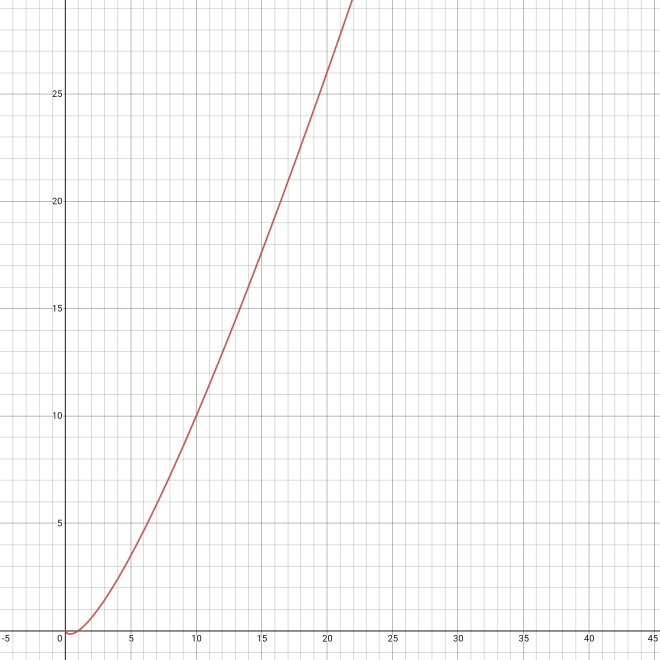
\includegraphics[width=3.0in,height=3.0in]{./media/image2.png}
	\end{Center}
\end{figure}


%%%%%%%%%%%%%%%%%%%% Figure/Image No: 2 Ends here %%%%%%%%%%%%%%%%%%%%


\vspace{\baselineskip}
\vspace{\baselineskip}
{\fontsize{9pt}{10.8pt}\selectfont \ \ \ \ \ \ \ \ \ \ \ \ \ \ \  Fig. 1 .Time complexity curve (N vs t) }

\vspace{\baselineskip}

\vspace{\baselineskip}

\vspace{\baselineskip}
\textbf{\ \ \ \ \ \ \ \ \ \ \ \  }\  

\vspace{\baselineskip}
{\fontsize{9pt}{10.8pt}\selectfont \ \ \ \ \ \ \ \ \ \ \ \ \ \ \ \  }\ \  {\fontsize{12pt}{14.4pt}\selectfont \textbf{V.} }{\fontsize{12pt}{14.4pt}\selectfont \textbf{C}}\textbf{ONCLUSION }

\vspace{\baselineskip}
In this paper we proposed an algorithm to find the\textcolor[HTML]{40424E}{,minimum computations done to reach Optimal Merge Pattern given n number of sorted files..}The experimental study showed that the time complexity of the algorithm using greedy programming is \textbf{O(n$\ast$ log(n)) }which depends on the number of the sorted files 

\vspace{\baselineskip}

\vspace{\baselineskip}

\vspace{\baselineskip}

\vspace{\baselineskip}

\vspace{\baselineskip}

\vspace{\baselineskip}
\textbf{\ \ \ \ \ \ \ \ \ \ \  \ \ \ \ \ \ \  }
\textbf{\ \  R}{\fontsize{8pt}{9.6pt}\selectfont \textbf{EFERENCES}}\textbf{\ \ \  }

\vspace{\baselineskip}
{\fontsize{9pt}{10.8pt}\selectfont \ \ \ \ \ [1]  \href{https://www.geeksforgeeks.org}{https://www.geeksforgeeks.org}}
{\fontsize{9pt}{10.8pt}\selectfont \ \ \ \ \ [2]  Introduction to Algorithms by Thomas H.cormen}
{\fontsize{9pt}{10.8pt}\selectfont \  }

\end{multicols}
\printbibliography
\end{document}